\documentclass[12pt, a4paper]{article}
\usepackage{../../../myconfig} % Gọi file cấu hình từ ngoài gốc vào

% ==========================================
% BẮT ĐẦU NỘI DUNG TÀI LIỆU
% ==========================================
\begin{document}

% Truyền 3 tham số: {Nhãn cam} {Chữ to chính giữa} {Chữ ở góc phải Header}
\titlebox{Chủ đề: định kì}{Đề kiểm tra định kì lần 4}{Đề định kì}

\textit{\textbf{Phần I: Thí sinh trả lời từ câu 1 đến câu 12, mỗi câu thí sinh chỉ chọn một phương án}}

\vspace{0.5cm}



% --- CÂU 1 ---
\questionLinesManual{0}{1}{Hàm số nào trong bốn hàm số được liệt kê dưới đây không có cực trị?}{%
    \begin{tasks}(4)
        \task \( y = \dfrac{2x - 3}{x + 2} \)
        \task \( y = x^4 \)
        \task \( y = -x^3 + x \)
        \task \( y = |x + 2| \)
    \end{tasks}
}

% --- CÂU 2 ---
\questionLinesManual{0}{2}{Với \( x \in [-\pi; \pi] \), phương trình \( \cos x = \dfrac{\sqrt{3}}{2} \) có bao nhiêu nghiệm?}{%
    \begin{tasks}(4)
        \task 1
        \task 2
        \task 3
        \task 4
    \end{tasks}
}

% --- CÂU 3 ---
\questionLinesManual{0}{3}{Cho cấp số nhân \( (u_n) \) có số hạng đầu \( u_1 = 5 \) và công bội \( q = -2 \). Tính \( S_6 \).}{%
    \begin{tasks}(4)
        \task \( S_6 = -\dfrac{155}{3} \)
        \task \( S_6 = -\dfrac{315}{3} \)
        \task \( S_6 = -315 \)
        \task \( S_6 = 315 \)
    \end{tasks}
}

% --- CÂU 4 ---
\questionLinesManual{0}{4}{Tập nghiệm của bất phương trình \( 10^{2x+3} \leq \dfrac{1}{10} \) là}{%
    \begin{tasks}(4)
        \task \((-2; +\infty)\)
        \task \((-\infty; -2)\)
        \task \((-\infty; -2]\)
        \task \([-2; +\infty)\)
    \end{tasks}
}

% --- CÂU 5 ---
\questionLinesManual{0}{5}{Nếu \( \displaystyle\int_{-3}^{1} f(x) \, dx = -2 \) thì \( \displaystyle\int_{-3}^{1} \left[ 2 - 5f(x) \right] \, dx \) bằng}{%
    \begin{tasks}(4)
        \task 18
        \task 6
        \task 12
        \task -4
    \end{tasks}
}

% --- CÂU 6 ---
\questionLinesManual{0}{6}{Cho hàm số \( y = \dfrac{x-1}{x+1} \) có đồ thị \( (C) \). Có bao nhiêu điểm thuộc đồ thị \( (C) \) sao cho tiếp tuyến của đồ thị \( (C) \) tại các điểm đó song song với đường thẳng \( y = 2x + 7 \)?}{%
    \begin{tasks}(4)
        \task 2
        \task 1
        \task 0
        \task 3
    \end{tasks}
}

% --- CÂU 7 ---
\questionLinesManual{0}{7}{Số giao điểm của đồ thị hàm số \( y = x^3 + 3x^2 \) và đồ thị hàm số \( y = 3x^2 + 3x \) là}{%
    \begin{tasks}(4)
        \task 3
        \task 1
        \task 2
        \task 0
    \end{tasks}
}

% --- CÂU 8 ---
\questionLinesManual{0}{8}{Cho hàm số \( y = f(x) \) có bảng xét dấu đạo hàm như sau:

\begin{center}

\begin{tikzpicture}
    \tkzTabInit[lgt=1.5, espcl=2.5]
    {$x$ /1, $f'(x)$ /1}
    {$-\infty$, $-1$, $0$, $1$, $+\infty$}
    \tkzTabLine{, -, d, -, 0, +, 0, -}
\end{tikzpicture}
\end{center}

Mệnh đề nào sau đây đúng?}{%
    \begin{tasks}(2)
        \task \(\max\limits_{(-1;1]} f(x) = f(0)\)
        \task \(\max\limits_{(0;+\infty)} f(x) = f(1)\)
        \task \(\min\limits_{(-\infty;-1]} f(x) = f(-1)\)
        \task \(\min\limits_{(-1;+\infty)} f(x) = f(0)\)
    \end{tasks}
}

% --- CÂU 9 ---
\questionLinesManual{0}{9}{Cho \( F(x) \) là một nguyên hàm của hàm số \( f(x) = e^x + 2x \) thỏa mãn \( F(0) = \dfrac{3}{2} \). Tìm \( F(x) \).}{%
    \begin{tasks}(2)
        \task \( F(x) = e^x + x^2 + \dfrac{1}{2} \)
        \task \( F(x) = e^x + x^2 + \dfrac{5}{2} \)
        \task \( F(x) = e^x + x^2 + \dfrac{3}{2} \)
        \task \( F(x) = 2e^x + x^2 - \dfrac{1}{2} \)
    \end{tasks}
}

% --- CÂU 10 ---
\questionLinesManual{0}{10}{Cho một vật thể giới hạn bởi hai mặt phẳng vuông góc với trục \( Ox \) tại các điểm có hoành độ \( x = -1 \) và \( x = 1 \). Một mặt phẳng vuông góc với trục \( Ox \) tại \( x(-1 \leq x \leq 1) \) cắt vật thể đó theo một mặt cắt là hình vuông có cạnh bằng \( \sqrt{1 - x^4} \). Thể tích của vật thể đó bằng}{%
    \begin{tasks}(4)
        \task \( \dfrac{4}{5} \)
        \task \( \dfrac{4\pi}{5} \)
        \task \( \dfrac{8}{5} \)
        \task \( \dfrac{8\pi}{5} \)
    \end{tasks}
}

% --- CÂU 11 ---
\questionLinesManual{0}{11}{Cho hàm số \( y = f(x) \) có đồ thị như hình vẽ

\begin{center}
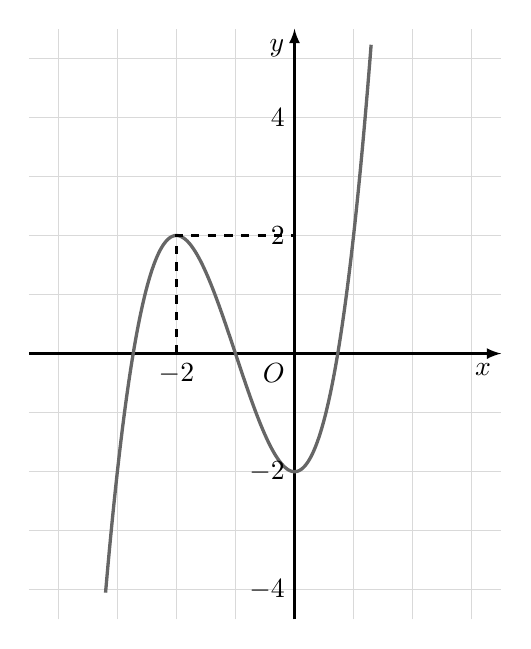
\begin{tikzpicture}[scale=0.75, >=latex]

    % 1. Lưới ô vuông
    \draw[gray!30, thin] (-4.5, -4.5) grid (3.5, 5.5);

    % 2. Trục tọa độ Ox, Oy
    \draw[->, thick] (-4.5, 0) -- (3.5, 0) node[below left] {$x$};
    \draw[->, thick] (0, -4.5) -- (0, 5.5) node[below left] {$y$};

    % Gốc tọa độ O
    \node[below left] at (0, 0) {$O$};

    % 3. Đồ thị hàm số bậc ba y = f(x) = 0.5*x^3 + 1.5*x^2 - 2
    % Cực đại tại (-2, 2) và cực tiểu tại (0, -2)
    \draw[very thick, gray!80!black, smooth, domain=-3.2:1.3, samples=200] 
        plot (\x, {\x*\x*\x + 3*\x*\x - 2});

    % 4. Các đường nét đứt cực trị (-2, 2)
    \draw[dashed, thick, black] (-2, 0) -- (-2, 2) -- (0, 2);

    % 5. Đánh dấu các nhãn số trên trục
    \node[below] at (-2, 0) {$-2$};
    \node[left] at (0, 2) {$2$};
    \node[left] at (0, -2) {$-2$};
    \node[left] at (0, -4) {$-4$};
    \node[left] at (0, 4) {$4$};

\end{tikzpicture}
\end{center}

Số tiệm cận đứng của đồ thị hàm số \( y = \dfrac{2019}{f(x) - 1} \) là}{%
    \begin{tasks}(4)
        \task 1
        \task 2
        \task 3
        \task 4
    \end{tasks}
}

% --- CÂU 12 ---
\questionLinesManual{0}{12}{Cho \( \displaystyle\int_{0}^{1} \left( \dfrac{1}{x+1} - \dfrac{1}{x+2} \right) dx = a \ln 2 + b \ln 3 \) với \(a, b\) là các số nguyên. Mệnh đề nào dưới đây đúng?}{%
    \begin{tasks}(4)
        \task \(a + 2b = 0\)
        \task \(a + b = 2\)
        \task \(a - 2b = 0\)
        \task \(a + b = -2\)
    \end{tasks}
}

\textit{\textbf{Phần II: Thí sinh trả lời từ câu 13 đến câu 16; trong mỗi ý a), b), c), d) ở mỗi câu, thí sinh chọn đúng hoặc sai.}}

\vspace{0.3cm}

\questionTrueFalse{0}{13}{Cho hàm số \( y = \sqrt{x+2} \) (\( x \geq -2 \)) và đường thẳng \( y = x \).
\begin{center}
    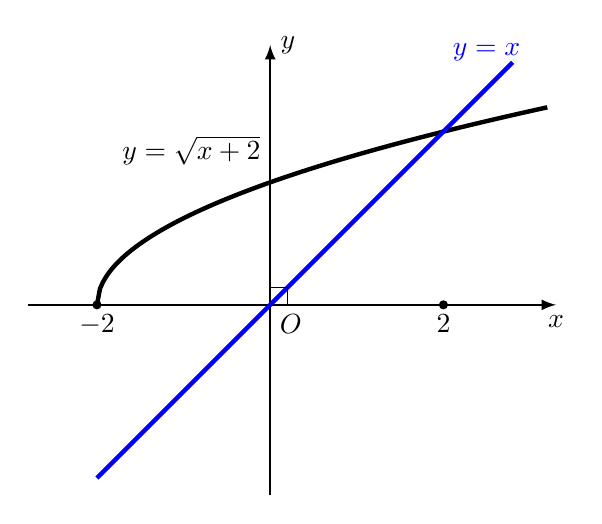
\begin{tikzpicture}[scale=1.1, >=latex]
    % Giới hạn vùng hiển thị bằng \clip
    \clip (-2.8, -2.2) rectangle (3.5, 3.2);

    % 1. Trục tọa độ Ox, Oy
    \draw[->, thick] (-2.8, 0) -- (3.3, 0) node[below] {$x$};
    \draw[->, thick] (0, -2.2) -- (0, 3.0) node[right] {$y$};
    \node[below right] at (0, 0) {$O$};

    % 2. Đồ thị hàm số y = sqrt(x + 2)
    \draw[ultra thick, black, domain=-2:3.2, samples=150] plot (\x, {sqrt(\x + 2)});
    \node[above left] at (0, 1.5) {$y = \sqrt{x+2}$};

    % 3. Đường thẳng y = x
    \draw[ultra thick, blue, domain=-2.0:2.8, samples=2] plot (\x, {\x});
    \node[above left, blue] at (3, 2.7) {$y = x$};

    % 4. Đánh dấu các điểm mốc trên trục Ox
    \fill[black] (-2, 0) circle (1.5pt) node[below] {$-2$};
    \fill[black] (2, 0) circle (1.5pt) node[below] {$2$};

    % 5. Ký hiệu góc vuông tại gốc tọa độ O
    \draw[thin] (0.2, 0) -- (0.2, 0.2) -- (0, 0.2);

\end{tikzpicture}
\end{center}
}{
    \textbf{a)} & Diện tích hình phẳng \( D \) giới hạn bởi đồ thị hàm số \( y = \sqrt{x+2} \) (\( x \geq -2 \)), trục tung, trục hoành và đường thẳng \( x = 2 \) là \( S_D = \dfrac{16}{3} - \dfrac{4\sqrt{2}}{3} \) (đvdt).
    & \textcolor{amberorange}{$\bigcirc$} & \textcolor{amberorange}{$\bigcirc$} \\ \hline
    
    \textbf{b)} & Diện tích hình phẳng giới hạn bởi đồ thị hàm số \( y = \sqrt{x+2} \) và đường thẳng \( y = x \), hai đường thẳng \( x = 0 \), \( x = 2 \) là \( S = \dfrac{10}{3} - \dfrac{2\sqrt{2}}{9} \) (đvdt).
    & \textcolor{amberorange}{$\bigcirc$} & \textcolor{amberorange}{$\bigcirc$} \\ \hline
    
    \textbf{c)} & Thể tích khối tròn xoay tạo thành khi quay hình phẳng giới hạn bởi đường thẳng \( y = x \), trục hoành, hai đường thẳng \( x = 1 \), \( x = 3 \) quanh trục \( Ox \) là \( 5\pi \) (đvtt).
    & \textcolor{amberorange}{$\bigcirc$} & \textcolor{amberorange}{$\bigcirc$} \\ \hline
    
    \textbf{d)} & Thể tích khối tròn xoay tạo thành khi quay hình phẳng \( D \) quanh trục \( Ox \) là \( 6\pi \) (đvtt).
    & \textcolor{amberorange}{$\bigcirc$} & \textcolor{amberorange}{$\bigcirc$} \\
}


\questionTrueFalse{0}{14}{Người ta bơm xăng vào bình xăng của một xe ô tô. Biết rằng thể tích \( V \) (tính theo lít) của lượng xăng trong bình xăng được tính theo thời gian bơm xăng \( t \) (phút) được cho bởi công thức:  
\(V(t) = 300 \left( t^2 - t^3 \right) + 4,5\)  
với \( 0 \leq t \leq 0,5 \).  

Gọi \( V'(t) \) là tốc độ tăng thể tích tại thời điểm \( t \) với \( 0 \leq t \leq 0,5 \). Biết 1 lít xăng có giá là 21.000 đồng.}{
    \textbf{a)} & Lượng xăng ban đầu trong bình là 1,5 lít.
    & \textcolor{amberorange}{$\bigcirc$} & \textcolor{amberorange}{$\bigcirc$} \\ \hline
    
    \textbf{b)} & Sau khi bơm 30 giây thì bình xăng đầy. Số tiền người mua phải trả là 787.500 đồng.
    & \textcolor{amberorange}{$\bigcirc$} & \textcolor{amberorange}{$\bigcirc$} \\ \hline
    
    \textbf{c)} & Khi xăng chảy vào bình xăng thì tốc độ tăng thể tích là lớn nhất vào thời điểm ở giây thứ 21.
    & \textcolor{amberorange}{$\bigcirc$} & \textcolor{amberorange}{$\bigcirc$} \\ \hline
    
    \textbf{d)} & Phương trình \(V'(t) = 0\) có hai nghiệm phân biệt trên đoạn \(\left[ 0; \dfrac{1}{2} \right]\).
    & \textcolor{amberorange}{$\bigcirc$} & \textcolor{amberorange}{$\bigcirc$} \\
}

\questionTrueFalse{0}{15}{Để loại bỏ \( x \) chất gây ô nhiễm không khí từ khí thải của một nhà máy, người ta ước tính chi phí cần bỏ ra là:  
\(C(x) = \dfrac{300x}{100 - x} \quad (\text{triệu đồng}) \quad 0 \leq x < 100.\)  
Xét tính đúng sai của mệnh đề sau:}{
    \textbf{a)} & \(C'(x) = -\dfrac{30000}{(100 - x)^2} \quad \text{với mọi } x \in [0; 100)\).
    & \textcolor{amberorange}{$\bigcirc$} & \textcolor{amberorange}{$\bigcirc$} \\ \hline
    
    \textbf{b)} & Để loại bỏ được 50\% chất gây ô nhiễm cần 300 triệu đồng.
    & \textcolor{amberorange}{$\bigcirc$} & \textcolor{amberorange}{$\bigcirc$} \\ \hline
    
    \textbf{c)} & Chi phí bỏ ra luôn tăng khi \( x \) tăng.
    & \textcolor{amberorange}{$\bigcirc$} & \textcolor{amberorange}{$\bigcirc$} \\ \hline
    
    \textbf{d)} & Không thể loại bỏ 100\% chất gây ô nhiễm dù bỏ ra chi phí là bao nhiêu đi chăng nữa.
    & \textcolor{amberorange}{$\bigcirc$} & \textcolor{amberorange}{$\bigcirc$} \\
}

\questionTrueFalse{0}{16}{Để tham gia lễ hội hóa trang, bạn An dự định làm một chiếc mặt nạ nửa mặt bằng chất liệu giấy cứng. Hình dạng của chiếc mặt nạ được bạn thiết kế trên mặt phẳng tọa độ \( Oxy \), là phần hình phẳng giới hạn bởi hai đường parabol \( (P_1), (P_2) \) lần lượt có đỉnh là gốc tọa độ \( O \) và điểm có tọa độ \( (0; 4) \), cùng nhận trục \( Oy \) làm trục đối xứng và cùng đi qua điểm \( M(5; 6) \). Mỗi đơn vị trên các trục tọa độ có độ dài 3 cm. Sau đó, bạn vẽ hai hình thoi bằng nhau có độ dài các đường chéo là \( 2\sqrt{2} \, \text{cm} \) và \( 4\sqrt{2} \, \text{cm} \) để khoét làm mắt.

\begin{center}
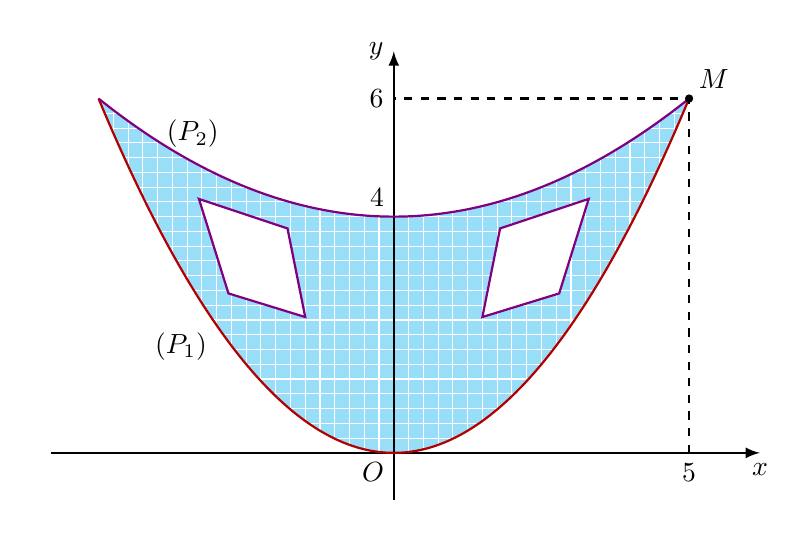
\begin{tikzpicture}[scale=0.75, >=latex]
    % Giới hạn vùng hiển thị bằng \clip
    \clip (-6.2, -1.2) rectangle (6.5, 7.2);

    % 1. Tô màu nền xanh có họa tiết lưới cho phần giới hạn giữa hai parabol
    \begin{scope}
        \clip plot[domain=-5:5, samples=100] (\x, {2/25*\x*\x + 4}) 
            -- plot[domain=5:-5, samples=100] (\x, {6/25*\x*\x}) -- cycle;
        
        % Đổ màu nền xanh nhạt
        \fill[cyan!40] (-6, -1) rectangle (6, 7);
        % Vẽ họa tiết lưới ô vuông
        \draw[step=0.25cm, white, thin] (-6, -1) grid (6, 7);

        % Đè hai mắt (hình thoi/tứ giác) bằng màu trắng
        \fill[white] (1.8, 3.8) -- (3.3, 4.3) -- (2.8, 2.7) -- (1.5, 2.3) -- cycle;
        \fill[white] (-1.8, 3.8) -- (-3.3, 4.3) -- (-2.8, 2.7) -- (-1.5, 2.3) -- cycle;
    \end{scope}

    % 2. Trục tọa độ Ox, Oy
    \draw[->, thick] (-5.8, 0) -- (6.2, 0) node[below] {$x$};
    \draw[->, thick] (0, -0.8) -- (0, 6.8) node[left] {$y$};
    \node[below left] at (0, 0) {$O$};

    % 3. Vẽ hai đường Parabol
    % Parabol P1 (đường nét đỏ ở dưới)
    \draw[thick, red!70!black, domain=-5:5, samples=120] plot (\x, {6/25*\x*\x});
    
    % Parabol P2 (đường nét tím/xanh ở trên)
    \draw[thick, violet, domain=-5:5, samples=120] plot (\x, {2/25*\x*\x + 4});

    % 4. Vẽ các mắt hình thoi (viền tím)
    \draw[thick, violet] (1.8, 3.8) -- (3.3, 4.3) -- (2.8, 2.7) -- (1.5, 2.3) -- cycle;
    \draw[thick, violet] (-1.8, 3.8) -- (-3.3, 4.3) -- (-2.8, 2.7) -- (-1.5, 2.3) -- cycle;

    % 5. Các đường nét đứt định vị điểm M(5, 6) và đỉnh (0, 4)
    \draw[dashed, thick] (5, 0) node[below] {$5$} -- (5, 6) -- (0, 6) node[left] {$6$};
    \fill[black] (5, 6) circle (2pt) node[above right] {$M$};
    
    \node[above left] at (0, 4) {$4$};

    % 6. Tên các đường Parabol
    \node[above left] at (-2.8, 5) {$(P_2)$};
    \node[below left] at (-3, 2.2) {$(P_1)$};

\end{tikzpicture}
\end{center}
}{
    \textbf{a)} & Diện tích hai hình thoi được khoét để làm mắt là: \( 16 \, \text{cm}^2 \).
    & \textcolor{amberorange}{$\bigcirc$} & \textcolor{amberorange}{$\bigcirc$} \\ \hline
    
    \textbf{b)} & Phương trình của parabol \( (P_1) \):  
    \( y = \dfrac{6}{25} x^2 \) và phương trình của parabol \( (P_2) \):  
    \( y = \dfrac{2}{25} x^2 + 4 \).
    & \textcolor{amberorange}{$\bigcirc$} & \textcolor{amberorange}{$\bigcirc$} \\ \hline
    
    \textbf{c)} & Diện tích phần hình phẳng giới hạn bởi \( (P_1) \) và \( (P_2) \) là: \(\dfrac{40}{3}\) (đơn vị diện tích).
    & \textcolor{amberorange}{$\bigcirc$} & \textcolor{amberorange}{$\bigcirc$} \\ \hline
    
    \textbf{d)} & Diện tích giấy được bạn An sử dụng để làm chiếc mặt nạ này là \( 224 \, \text{cm}^2 \).
    & \textcolor{amberorange}{$\bigcirc$} & \textcolor{amberorange}{$\bigcirc$} \\
}

\textit{\textbf{Phần III: Thí sinh trả lời từ câu 17 đến câu 22.}}

\vspace{0.3cm}

\questionShortAnswer{0}{17}{Một doanh nghiệp dự định sản xuất không quá 300 sản phẩm.  
Nếu doanh nghiệp sản xuất \( x \) sản phẩm (\( 1 \leq x \leq 300 \)) thì doanh thu nhận được khi bán hết số sản phẩm đó là  
\( F(x) = -2x^2 + 1312x \) (nghìn đồng), trong khi chi phí sản xuất bình quân cho một sản phẩm là  
\( G(x) = x^2 - 77x + 1000 + \dfrac{40000}{x} \) (nghìn đồng). Lợi nhuận thu được của doanh nghiệp (tính theo đơn vị triệu đồng) đạt giá trị lớn nhất bằng bao nhiêu (làm tròn kết quả đến hàng đơn vị).
}

\questionShortAnswer{0}{18}{Trên cửa sổ có dạng hình chữ nhật của ngôi nhà một doanh nghiệp kinh doanh hải sản, họa sĩ cần thiết kế logo hình con cá. Logo là hình phẳng giới hạn bởi hai parabol với các kích thước được cho trong hình bên dưới (đơn vị trên mỗi trục tọa độ là \( dm \)). Họa sĩ cần tính diện tích của logo để báo giá cho doanh nghiệp đó trước khi kí hợp đồng. Diện tích của logo bằng \( x \, dm^2 \). Tìm \( x \) (kết quả làm tròn đến hàng đơn vị).

\begin{center}
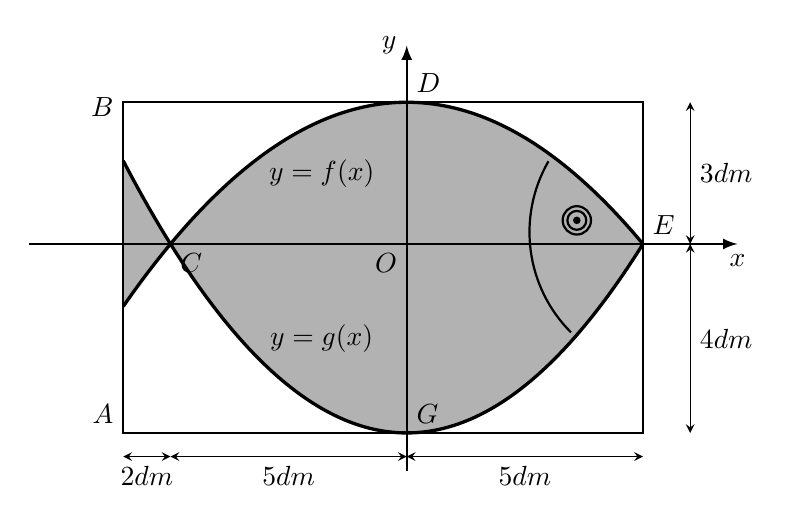
\begin{tikzpicture}[scale=0.6, >=latex]
    % Phần thân cá (từ x = -5 đến x = 5)
    \fill[gray!60] plot[domain=-5:5, samples=100] (\x, {-3/25*\x*\x + 3})
        -- plot[domain=5:-5, samples=100] (\x, {4/25*\x*\x - 4}) -- cycle;

    % Phần đuôi cá (từ x = -7 đến x = -5)
    \fill[gray!60] plot[domain=-6:-5, samples=100] (\x, {4/25*\x*\x - 4})
        -- (-5, 0) -- plot[domain=-5:-6, samples=100] (\x, {-3/25*\x*\x + 3}) -- cycle;

    % 2. Khung hình chữ nhật ngoài
    \draw[thick] (-6, -4) rectangle (5, 3);

    % 3. Trục tọa độ Ox, Oy
    \draw[->, thick] (-8, 0) -- (7, 0) node[below] {$x$};
    \draw[->, thick] (0, -4.8) -- (0, 4.2) node[left] {$y$};
    \node[below left] at (0, 0) {$O$};

    % 4. Vẽ hai đường Parabol
    % y = f(x)
    \draw[very thick, domain=-6:5, samples=100] plot (\x, {-3/25*(\x-5)*(\x+5)});
    % y = g(x)
    \draw[very thick, domain=-6:5, samples=100] plot (\x, {4/25*(\x-5)*(\x+5)});

    % 5. Cung tròn mang cá và mắt cá
    \draw[thick] (3, 1.75) arc [start angle=150, end angle=225, radius=3];
    
    % ĐÃ SỬA: Vẽ mắt cá đúng cú pháp
    \draw[fill=gray!60, thick] (3.6, 0.5) circle (0.2cm);  % ĐÃ SỬA
    \fill[black] (3.6, 0.5) circle (0.08cm);
    \draw[thick] (3.6, 0.5) circle (0.3cm);

    % 6. Tên các đỉnh/điểm mốc
    \node[below left] at (-6, -3.2) {$A$};
    \node[above left] at (-6, 2.5) {$B$};
    \node[below right] at (-5, 0) {$C$};
    \node[above right] at (0, 3) {$D$};
    \node[above right] at (5, 0) {$E$};
    \node[above right] at (0, -4) {$G$};

    % 7. Nhãn công thức hàm số
    \node[above] at (-1.8, 1) {$y=f(x)$};
    \node[below] at (-1.8, -1.5) {$y=g(x)$};

    % 8. Kích thước và mũi tên đo đạc
    % Bên phải
    \draw[<->, >=stealth, thin] (6, 0) -- (6, 3);
    \node[right] at (6, 1.5) {$3\text{dm}$};
    
    \draw[<->, >=stealth, thin] (6, -4) -- (6, 0);
    \node[right] at (6, -2) {$4\text{dm}$};

    % Bên dưới
    \draw[<->, >=stealth, thin] (-6, -4.5) -- (-5, -4.5);
    \node[below] at (-5.5, -4.5) {$2\text{dm}$};

    \draw[<->, >=stealth, thin] (-5, -4.5) -- (0, -4.5);
    \node[below] at (-2.5, -4.5) {$5\text{dm}$};

    \draw[<->, >=stealth, thin] (0, -4.5) -- (5, -4.5);
    \node[below] at (2.5, -4.5) {$5\text{dm}$};

\end{tikzpicture}
\end{center}
}

\questionShortAnswer{0}{19}{Cho một bờ hồ hình bán nguyệt có bán kính bằng \( 4km \), đường kính \( PR \) như hình vẽ sau:

\begin{center}
\begin{tikzpicture}[scale=0.9, >=stealth]
    % Giới hạn vùng hiển thị
    \clip (-4.8, -1.2) rectangle (4.8, 4.8);

    % 1. Đất bên dưới đường kính PR (gạch chéo)
    \fill[pattern=north east lines, pattern color=gray!80] (-4.2, -0.3) rectangle (4.2, 0);

    % 2. Bờ hồ hình bán nguyệt
    \draw[very thick] (4, 0) arc [start angle=0, end angle=180, radius=4];
    \draw[very thick] (-4, 0) -- (4, 0);

    % 3. Các đường nối PQ (chèo thuyền), QR (chạy bộ), QR nét đứt, OQ
    \draw[thick] (-4, 0) -- (1.5, 3.708); % PQ
    \draw[thick, dashed] (1.5, 3.708) -- (4, 0); % QR thẳng

    % Mũi tên chỉ hướng chèo thuyền PQ
    \draw[thick, ->] (-4, 0) -- (-1.25, 1.854);

    % Mũi tên chỉ hướng chạy bộ dọc cung QR
    \draw[thick, ->] (1.5, 3.708) arc [start angle=67.97, end angle=30, radius=4];

    % 4. Các điểm mốc P, Q, R, O
    \fill[black] (-4, 0) circle (2.5pt) node[below left, font=\large] {$P$};
    \fill[black] (4, 0) circle (2.5pt) node[below right, font=\large] {$R$};
    \fill[black] (0, 0) circle (2.5pt) node[below, font=\large] {$O$};
    \fill[black] (1.5, 3.708) circle (2.5pt) node[above, font=\large] {$Q$};

\end{tikzpicture}
\end{center}

Từ điểm \( P \) anh Bắp chèo một chiếc thuyền với vận tốc \( 5 \, km/h \) đến điểm \( Q \) trên bờ hồ, rồi chạy bộ dọc theo thành hồ đến vị trí \( R \) với vận tốc \( 8 \, km/h \). Thời gian lớn nhất mà anh Bắp đi chuyển từ \( P \) đến \( R \) là bao nhiêu (thời gian tính bằng giờ, kết quả làm tròn đến hàng phần trăm)?


}

\questionShortAnswer{0}{20}{Một bình gốm (có dạng như hình vẽ) có đường kính đáy là 20cm, đường kính lớn nhất của thân thùng là 36cm, chiều cao thùng là 50cm, cạnh bên hông của thùng có hình dạng của một parabol. Thể tích của bình gốm đó là bao nhiêu lít (kết quả làm tròn đến hàng phần chục).

\begin{center}
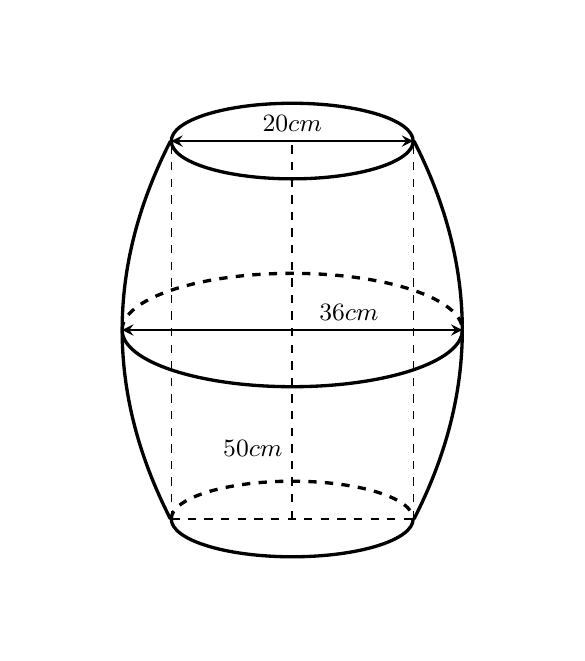
\begin{tikzpicture}[scale=0.12 , >=latex]
    % Giới hạn vùng hiển thị
    \clip (-28, -32) rectangle (28, 32);

    % 1. Vẽ thân bình gốm (2 đường parabol hai bên)
    \draw[very thick] plot[domain=-20:20, samples=100] ({-8/625*\x*\x + 18}, \x);
    \draw[very thick] plot[domain=-20:20, samples=100] ({-( -8/625*\x*\x + 18)}, \x);

    % 2. Mặt đáy trên (elip đầy đủ)
    \draw[very thick] (0, 20) ellipse (12.8cm and 4cm);

    % 3. Đường xích đạo giữa (nửa sau nét đứt, nửa trước nét liền)
    \draw[very thick, dashed] (-18, 0) arc [start angle=180, end angle=0, x radius=18, y radius=6];
    \draw[very thick] (-18, 0) arc [start angle=180, end angle=360, x radius=18, y radius=6];

    % 4. Mặt đáy dưới (nửa sau nét đứt, nửa trước nét liền)
    \draw[very thick, dashed] (-12.8, -20) arc [start angle=180, end angle=0, x radius=12.8, y radius=4];
    \draw[very thick] (-12.8, -20) arc [start angle=180, end angle=360, x radius=12.8, y radius=4];

    % 5. Trục đối xứng giữa (nét đứt) và các nét gióng đứng
    \draw[dashed, thick] (0, -20) -- (0, 20);
    \draw[dashed, thin] (-12.8, -20) -- (-12.8, 20);
    \draw[dashed, thin] (12.8, -20) -- (12.8, 20);
    \draw[dashed, thin] (-12.8, -20) -- (12.8, -20);
    % 6. Các kích thước và mũi tên đo đạc
    % Đường kính đáy trên: 20cm
    \draw[<->, >=stealth, thick] (-12.8, 20) -- (12.8, 20);
    \node[above, font=\small] at (0, 20) {$20\text{ cm}$};

    % Đường kính giữa: 36cm
    \draw[<->, >=stealth, thick] (-18, 0) -- (18, 0);
    \node[above, font=\small] at (6, 0) {$36\text{ cm}$};

    % Chiều cao: 50cm
    
    \node[left, font=\small] at (0, -12.5) {$50\text{ cm}$};

\end{tikzpicture}
\end{center}
}

\questionShortAnswer{0}{21}{Khi sản xuất vỏ lon sữa DUTCH LADY, các nhà sản xuất luôn đặt tiêu chí sao cho chi phí sản xuất vỏ lon là nhỏ nhất. Biết rằng lon sữa có hình trụ và thể tích của lon sữa là \( 530 \, \text{cm}^3 \). Khi diện tích toàn phần của lon sữa nhỏ nhất thì bán kính đáy của nó bằng bao nhiêu centimet? (làm tròn kết quả đến hàng phần trăm)
\begin{figure}[H]
    \centering
    
\includegraphics[width=0.3\textwidth]{images/LonSua.png}
\end{figure}

}

\questionShortAnswer{0}{22}{Một máng nước có thiết diện là một hình thang cân, với các kích thước của máng được cho như trong hình vẽ. Nước được bơm vào máng với tốc độ là 4 lít/phút. Hỏi tốc độ dâng lên của mực nước vào thời điểm mà mực nước trong máng cao \( 2dm \) là bao nhiêu dm/phút (\( t = 0 \) là lúc bắt đầu bơm nước) (kết quả làm tròn đến hàng phần trăm)?

\begin{center}
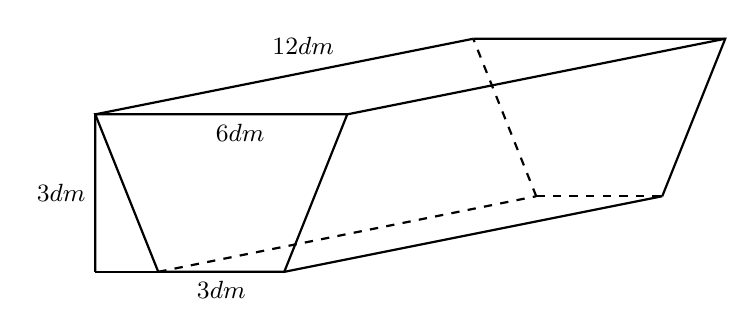
\begin{tikzpicture}[scale=0.8, >=stealth]
      % Mặt trước (hình thang cân)
    \coordinate (A) at (-1.5, 0);   % Đáy nhỏ trái
    \coordinate (B) at (0.5, 0);    % Đáy nhỏ phải
    \coordinate (C) at (1.5, 2.5);  % Đáy lớn phải
    \coordinate (D) at (-2.5, 2.5); % Đáy lớn trái

    % Mặt sau (dịch chuyển theo véc-tơ (6, 1.2))
    \coordinate (A') at (4.5, 1.2);
    \coordinate (B') at (6.5, 1.2);
    \coordinate (C') at (7.5, 3.7);
    \coordinate (D') at (3.5, 3.7);

    % 1. Các cạnh nét đứt (bị che khuất)
    \draw[thick, dashed] (A) -- (A');
    \draw[thick, dashed] (A') -- (B');
    \draw[thick, dashed] (A') -- (D');

    % 2. Các cạnh nét liền (nhìn thấy)
    \draw[thick] (A) -- (B) -- (C) -- (D) -- cycle; % Mặt trước
    \draw[thick] (B) -- (B');
    \draw[thick] (C) -- (C');
    \draw[thick] (D) -- (D');
    \draw[thick] (B') -- (C') -- (D'); % Mặt sau

    % 3. Đường cao thiết diện
    \draw[thick] (D) -- (-2.5, 0);
    \draw[thick] (-2.5, 0) -- (A);

    % 4. Các nhãn kích thước
    \node[above, font=\small] at (0.8, 3.3) {$12\text{dm}$};
    \node[below, font=\small] at (-0.2, 2.5) {$6\text{dm}$};
    \node[below, font=\small] at (-0.5, 0) {$3\text{dm}$};
    \node[left, font=\small] at (-2.5, 1.25) {$3\text{dm}$};

\end{tikzpicture}
\end{center}
}

\end{document}